\documentclass[a4paper]{article}

\usepackage[spanish]{babel}
\usepackage[utf8]{inputenc}
\usepackage{amsmath}
\usepackage{graphicx}
\usepackage{epigraph}
\usepackage[colorinlistoftodos]{todonotes}
\setlength{\parskip}{3mm}
\title{Nociones de la memoria del computador}
\setlength\parindent{0pt}
\usepackage{times}		
\usepackage[T1]{fontenc}

\author{Sebastián Marulanda Quiceno}

\date{Septiembre Del 2020}

\begin{document}
\maketitle

\epigraph{Si no sabes una verdad en su totalidad, entonces eres preso de una mentira.}{Proverbio de autor anonimo}


\section{Defina que es la memoria del computador.}

Una memoria es como un cerebro humano. Se utiliza para almacenar datos e instrucciones. la memoria de la computadora es el espacio de almacenamiento en la computadora donde los datos van a ser procesados y se almacenan las instrucciones necesarias para el procesamiento. 

La memoria es uno de los componentes fundamentales para el correcto funcionamiento de nuestra PC, ya que su existencia permite que la computadora pueda arrancar, se procesen los datos, se ejecuten las instrucciones para los distintos programas y demás. Por otro lado, cuanto mayor es la cantidad de memoria que posea una PC, mayor será el rendimiento y la mejora en la performance del equipo. Una computadora trabaja con cuatro tipos de memorias diferentes, que sirven para realizar diversas funciones. Estas son la memoria RAM, la memoria ROM, la memoria SRAM o Caché y la memoria Virtual o de Swap.


\section{Mencione los tipos de memoria que conoce y haga una pequeña descripción de cada tipo.}
\label{sec:examples}

\subsection{Disco duro}

    \begin{center}
    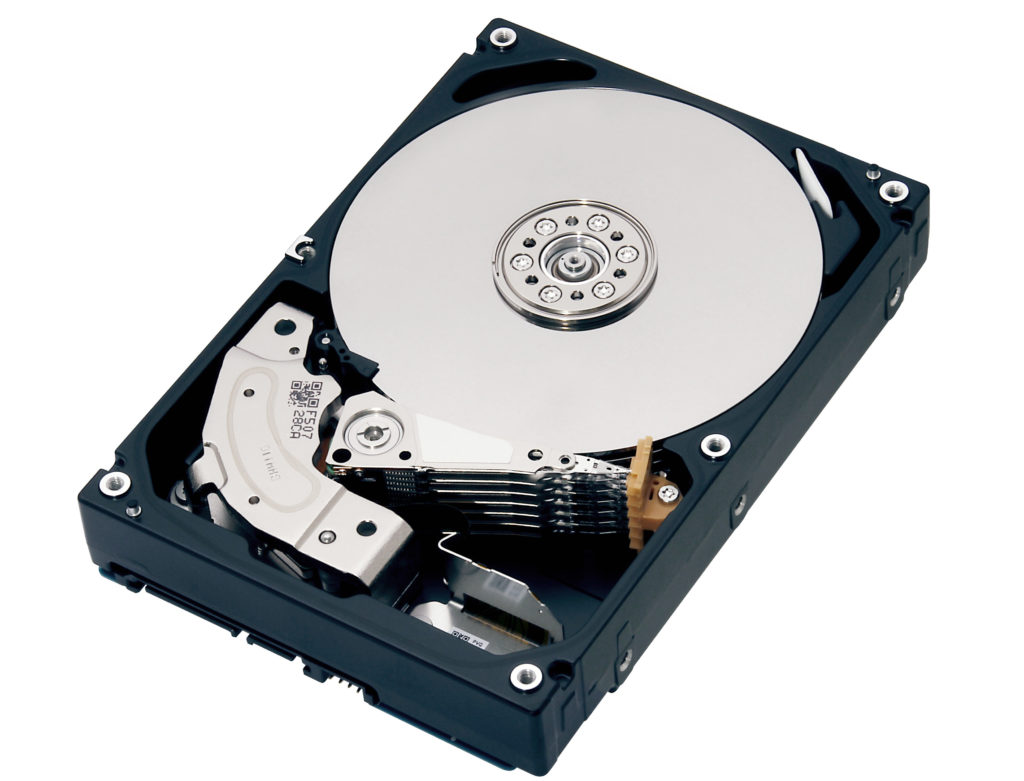
\includegraphics[width=0.3\textwidth]{images/discoduro.jpg}
    \end{center}
    
Un disco duro es un dispositivo para el almacenamiento de datos de forma no volátil, es decir, para almacenar los datos digitales utiliza un sistema de grabación magnética. tambien existen los discos duros de estado solido que son una alternativa a los discos duros. La gran diferencia es que mientras los discos duros utilizan componentes mecánicos que se mueven, las SSD almacenan los archivos en microchips con memorias flash interconectadas entre sí.

\subsection{Memoria RAM}

    \begin{center}
    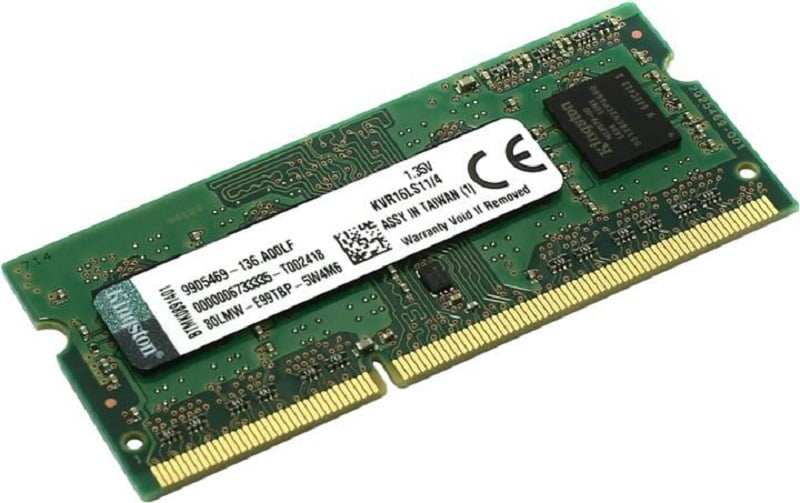
\includegraphics[width=0.3\textwidth]{images/ram.jpg}
    \end{center}

La memoria RAM o “memoria de acceso aleatorio” es la memoria principal del dispositivo, en la que se almacenan programas y datos. Sus siglas significan Random Access Memory y es el lugar en el que se cargan todas las instrucciones que ejecuta la unidad central de procesamiento y otras unidades del PC. La memoria RAM o aleatoria, también conocida como memoria volátil, no guarda los datos de manera permanente, es decir, que cuando deja de existir la fuente de energía en el dispositivo, la información se pierde.

\subsection{Memoria cache}

    \begin{center}
    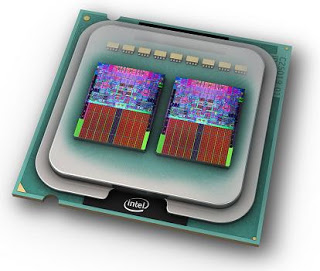
\includegraphics[width=0.3\textwidth]{images/cache.jpg}
    \end{center}
    
La memoria caché es una memoria de semiconductor de muy alta velocidad que puede acelerar el CPU. Actúa como un amortiguador entre la CPU y la memoria principal. Se utiliza para sostener las partes del programa y datos que se utilizan con mayor frecuencia por la CPU. Las partes de datos y programas se transfieren desde el disco a memoria caché por sistema operativo, desde donde CPU puede acceder a ellas.

\section{Describa la manera como se gestiona la memoria en un computador.}

La parte del sistema operativo que administra la memoria se llama administrador de memoria y su labor consiste en llevar un registro de las partes de memoria que se estén utilizando y aquellas que no, con el fin de asignar espacio en memoria a los procesos cuando éstos la necesiten y liberándola cuando terminen. De forma simplificada se trata de proveer mecanismos para asignar secciones de memoria a los programas que las solicitan, y a la vez, liberar las secciones de memoria que ya no se utilizan para que estén disponibles para otros programas.

Gestionar la memoria es importante para poder optimizar el espacio y poder cargar o intercambiar los programas que van hacer ejecutados del disco duro a la memoria principal. también el administrador de memoria se encarga de llevar un registro de las partes de la memoria que están en uso y de las que no. Si detecta que hay una parte que ya no está en uso, la libera para poder asignarla a los procesos que la necesiten. Y el administrador de memoria proporciona  protección y uso compartido, es decir, facilitar un espacio de memoria para cada proceso y controlar que ninguno de ellos trabaje en zonas de memoria que no le han sido asignados.

\section{¿Qué hace que una memoria sea más rápida que otra? ¿Por qué esto es importante?}

La velocidad de la memoria depende de muchos factores, de sus materiales, su numero de ceulas, su funcion, la temperatura. son demasiados parametros, por ejemplo la memoria RAM es mucho mas rapida que la ROM pero por que son para cosas diferentes, una es aleatoria y no guarda la informacion permanentemente y la otra es lo contrario, la temperatura tambien siempre ha sido un factor en la rapidez en los componentes de la computadora, y tambien afecta a la memoria, de todos estos factores depende de la velocidad de lectura y escriruta por segundo de las memorias.

La velocidad de la memoria es muy importante por que de esto depende la velocidad del computador, mientras mas rapido la memoria escriba y lea los datos mas rapido el computador los va a procesar, por eso si se tiene un computador con un disco duro SSD (que son mas rapidos que los HDD) el computador en si va a funcionar mas rapido que si tienes un HDD, entonces es importante su velocidad, para un buen funcionamiento del computador.

\end{document}